\documentclass[11pt]{article}
\usepackage[T1]{fontenc}
\usepackage[utf8]{inputenc}
\usepackage{lmodern}
\usepackage[margin=1in]{geometry}
\usepackage{amsmath,amssymb,amsthm,mathtools}
\usepackage{microtype,booktabs,array}
\usepackage{tikz}
\usetikzlibrary{arrows.meta}
\usepackage[hidelinks]{hyperref}
\hypersetup{pdftitle={The Partitioning of Power Sets Into Graphs},pdfsubject={Cyclic symmetric difference, binary necklaces, and functional graphs}}
\newtheorem{theorem}{Theorem}[section]
\newtheorem{proposition}[theorem]{Proposition}
\newtheorem{lemma}[theorem]{Lemma}
\newtheorem{corollary}[theorem]{Corollary}
\theoremstyle{definition}
\newtheorem{definition}[theorem]{Definition}
\newtheorem{example}[theorem]{Example}
\theoremstyle{remark}
\newtheorem{remark}[theorem]{Remark}
\numberwithin{equation}{section}
\newcommand{\F}{\mathbb F_2}
\newcommand{\Z}{\mathbb Z}
\newcommand{\N}{\mathbb Z_{>0}}
\newcommand{\G}{\mathcal G}
\newcommand{\Q}{\mathcal Q}
\newcommand{\phip}{\Phi}
\DeclareMathOperator{\ord}{ord}
\DeclareMathOperator{\lcm}{lcm}
\DeclareMathOperator{\Ann}{Ann}
\DeclareMathOperator{\im}{im}
\DeclareMathOperator{\Fix}{Fix}
\DeclareMathOperator{\height}{ht}
\allowdisplaybreaks[1]
\setlength{\emergencystretch}{2em}
\title{The Partitioning of Power Sets Into Graphs}
\author{}
\date{}

\begin{document}
\maketitle
\vspace{-2.5em}
\begin{abstract}
Let a cyclic permutation act on the power set of an $n$-element set, and let
evolution be symmetric difference with the cyclic translate. Since these
operations commute, evolution induces a functional graph on the rotation
classes of subsets. Its connected components induce a partition of the power
set. We give a self-contained algebraic description of the component types,
their multiplicities, and the cardinalities of the corresponding parts.
Writing $n=2^a m$ with $m$ odd, we separate a nilpotent coordinate from an
invertible periodic coordinate. Every component is a directed cycle with
identical level-regular rooted trees attached. Its cycle length determines
its tree shape at fixed $n$. Simultaneous rotation and evolution relations
form a rank-two integer lattice; passing from squarefree factors to repeated
factors multiplies this lattice by a power of two. Consequently, finitely many
integer polynomials associated with an odd $m$ describe the partitions for
every $m2^a$. Powers of two and the families $3\cdot2^a$, $5\cdot2^a$, and
$7\cdot2^a$ admit explicit formulas. A second description, using rotation
averaging and two M\"obius inversions, expresses all component multiplicities
through polynomial greatest common divisors. Both descriptions establish
disjointness and exhaustiveness without choosing individual subsets.
\end{abstract}

\noindent\textbf{Keywords.} Power sets; binary necklaces; Ducci map; additive
cellular automata; functional graphs; finite fields; M\"obius inversion.

\section{Introduction and definitions}\label{sec:introduction}

Let $X_n=\Z/n\Z$, with cyclic permutation $i\mapsto i+1$. For
$A\subseteq X_n$, write $R(A)=\{i+1:i\in A\}$ and define
\begin{equation}\label{eq:set-map}
 D(A)=A\mathbin{\triangle}R(A),
\end{equation}
where $\triangle$ denotes symmetric difference. The cyclic order is part of
the structure; different cyclic labelings give isomorphic constructions.
Under characteristic vectors, $\mathcal P(X_n)$ is the vector
space $V_n=\F^n$, rotation is a linear map $R$, and $D=I+R$.

A \emph{necklace} is an orbit under $\langle R\rangle$. Let
$\mathcal N_n=V_n/\langle R\rangle$, with projection $\pi_n$. Since $DR=RD$,
the rule $[v]\mapsto[Dv]$ defines a map $\overline D$ on $\mathcal N_n$.
Let $\Q_n$ be its functional digraph: every necklace is a vertex, and its
unique outgoing edge points to its image under $\overline D$. Loops are
retained. A \emph{component} means a weakly connected component, obtained by
ignoring edge directions when testing connectivity. Each component consists
of one directed cycle and trees directed toward that cycle.

For a component $C$ of $\Q_n$, define its \emph{mass} by
\begin{equation}\label{eq:mass}
 \lVert C\rVert=|\pi_n^{-1}(V(C))|.
\end{equation}
The sets $\pi_n^{-1}(V(C))$ partition $\mathcal P(X_n)$. This is the sense in
which the power set is partitioned into graphs: graph vertices are rotation
classes, while each part of the power set is their union. The number of
vertices in a component and its mass are different quantities. Isomorphic
components need not have the same mass.

The map $D$ is the binary Ducci map, within the theory of additive cellular
automata. Martin, Odlyzko, and Wolfram developed polynomial methods and
algebraic descriptions of finite state-transition graphs
\cite{MartinOdlyzkoWolfram}. Misiurewicz, Stevens, and Thomas studied
iterations of related linear maps over finite fields, including the passage
from dimension $n$ to dimension $2n$ and counts of periodic vectors
\cite{MisiurewiczStevensThomas}. Breuer, L\"otter, and van der Merwe related
Ducci periods to polynomial orders and multiplicative orders in finite fields
\cite{BreuerLotterMerwe}. The emphasis here is the quotient by cyclic rotation
and the simultaneous relations between rotation and evolution. All structural
and counting statements needed for this quotient are proved below.

Throughout, write uniquely
\begin{equation}\label{eq:decomposition}
 n=qm,\qquad q=2^a,\qquad a\in\Z_{\ge0},\qquad m\text{ odd}.
\end{equation}
Thus $a=v_2(n)$ is the exponent of $2$ in $n$. The main results are as follows.
The component classification in Theorem~\ref{thm:classification} identifies
every component through a polynomial divisor and a coset of a finite group.
Theorem~\ref{thm:trees} gives its complete directed-graph shape.
The lattice lifting theorem, Theorem~\ref{thm:lift}, yields the finite
polynomial description of all $m2^a$ in Theorem~\ref{thm:tower}.
Finally, Theorem~\ref{thm:mobius} gives an independent counting formula for
every positive integer $n$.

\section{The algebraic partition}\label{sec:partition}

\subsection{Nilpotent and periodic coordinates}

Identify $V_n$ with $\F[x]/(x^n+1)$ by sending a vector to its coordinate
polynomial. Then $R$ and $D$ act by multiplication by $x$ and $1+x$,
respectively. Put
\begin{equation}\label{eq:qm}
 Q_m(x)=\frac{x^m+1}{x+1},\qquad P_n(x)=Q_m(x)^q.
\end{equation}
For $m=1$, $Q_m=P_n=1$. Since $m$ is odd, $x^m+1$ is squarefree, and
$Q_m$ is relatively prime to $x(x+1)$. Moreover,
\begin{equation}\label{eq:crt}
 x^n+1=(x+1)^q Q_m(x)^q,\qquad
 V_n\simeq K_q\oplus W_n,
\end{equation}
where
\[
 K_q=\F[y]/(y^q),\quad y=x+1,
 \qquad W_n=\F[x]/P_n(x).
\]
The quotient by the polynomial $1$ is understood as the zero vector space.
On $K_q$, rotation is multiplication by $1+y$ and evolution by $y$.
On $W_n$, both $x$ and $1+x$ are units. Thus $K_q$ is the nilpotent part,
and $W_n$ is the periodic part. In particular, a vector is periodic under
$D$ exactly when its $K_q$ coordinate is zero.

\subsection{Annihilator strata and relation lattices}

For $w\in W_n$, its \emph{annihilator polynomial} is the monic generator
$H$ of $\{f\in\F[x]:fw=0\}$; necessarily $H\mid P_n$. Set
\[
 W_n(H)=\{w\in W_n:\Ann(w)=(H)\}.
\]
If $P_n=BH$, multiplication by $B$ identifies $W_n(H)$ with
\begin{equation}\label{eq:unit-stratum}
 U(H)=(\F[x]/H)^\times.
\end{equation}
Indeed $w=Bu$ has annihilator $H$ precisely when $\gcd(u,H)=1$.
For $H=1$, the stratum is $\{0\}$; we use a one-element group as $U(1)$.
Write
\begin{equation}\label{eq:phi-polynomial}
 \phip(H)=|U(H)|,
 \qquad
 \phip\left(\prod_i f_i^{e_i}\right)
 =\prod_i (2^{\deg f_i}-1)2^{(e_i-1)\deg f_i},
 \qquad \phip(1)=1.
\end{equation}

For $H\ne1$, define
\begin{equation}\label{eq:lattice}
 \Lambda_H=\{(u,v)\in\Z^2:x^u(1+x)^v=1\pmod H\}.
\end{equation}
Negative exponents are permitted because $x$ and $1+x$ are units.
There are unique integers $d_H,t_H>0$ and $0\le s_H<d_H$ such that
\begin{equation}\label{eq:lattice-basis}
 \Lambda_H=\langle(d_H,0),(-s_H,t_H)\rangle.
\end{equation}
Here $d_H$ is the order of $x$ modulo $H$, $t_H$ is the least positive
integer for which $(1+x)^{t_H}\in\langle x\rangle$, and
$(1+x)^{t_H}=x^{s_H}$. Since $H\mid x^n+1$, $d_H\mid n$.
The subgroup
\[
 \Gamma_H=\langle x,1+x\rangle\le U(H)
\]
has order $d_Ht_H$, by the homomorphism from $\Z^2$ with kernel
$\Lambda_H$. For $H=1$, set $(d_H,t_H,s_H)=(1,1,0)$ and take
$\Gamma_H$ to be trivial.

\begin{theorem}[Component classification]\label{thm:classification}
The components of $\Q_n$ are in bijection with the disjoint union
\begin{equation}\label{eq:coset-partition}
 \bigsqcup_{H\mid P_n} U(H)/\Gamma_H.
\end{equation}
For a fixed $H$, there are $\phip(H)/(d_Ht_H)$ components. Each has a
cycle of length $t_H$, and its mass is $2^q d_Ht_H$.
Consequently,
\begin{equation}\label{eq:stratum-coverage}
 \sum_{H\mid P_n}\frac{\phip(H)}{d_Ht_H}\,2^q d_Ht_H=2^n.
\end{equation}
\end{theorem}

\begin{proof}
Both $R$ and $D$ preserve each annihilator stratum and act on it as
multiplication by $x$ and $1+x$. Their joint orbits are precisely the
cosets of $\Gamma_H$, each of size $d_Ht_H$. Quotienting such an orbit by
rotation leaves $t_H$ vertices, on which $D$ acts as one cycle.

Every vector with periodic coordinate in this joint orbit reaches that
cycle after at most $q$ applications of $D$, because $y^q=0$ on $K_q$.
Conversely, neither a rotation nor an evolution edge can move the periodic
coordinate to a different joint orbit. Thus all $2^q d_Ht_H$ vectors in
the product of $K_q$ with the joint orbit form the inverse image of exactly
one component. This proves the asserted bijection and mass.

The CRT coordinates, annihilator polynomial, and coset are unique, proving
disjointness. They exhaust $V_n$, proving exhaustiveness. Equivalently,
$\sum_{H\mid P_n}\phip(H)=2^{\deg P_n}=2^{n-q}$, which gives
\eqref{eq:stratum-coverage}.
\end{proof}

\section{The directed-graph structure}\label{sec:trees}

For powers of two $h\mid q$, let $\mathcal T(q,h)$ be the rooted tree of
depth $q$ defined as follows. The root has one child. At depth $j$, where
$1\le j<q$, every vertex has
\begin{equation}\label{eq:branching}
 b_j(q,h)=
 \begin{cases}
 1,&j\in\{h,2h,4h,\ldots,q/2\},\\
 2,&\text{otherwise}
 \end{cases}
\end{equation}
children. The set in the first line is empty if $h=q$. All edges point
toward the root. Let $\G(T;q,h)$ be a directed cycle of length $T$ with
a copy of $\mathcal T(q,h)$ attached at each cycle vertex, identifying its
root with that vertex. For $T=1$ the cycle is a loop.

This specifies the graph up to isomorphism. An optional finite-word
encoding is
\begin{equation}\label{eq:branching-sequence}
 G_T\text{-}\sigma(q,h),\qquad
 \sigma(q,h)=2b_1(q,h)\cdots b_{q-1}(q,h)0.
\end{equation}
Juxtaposition in $\sigma(q,h)$ denotes concatenation in a word over $\{0,1,2\}$. The initial
symbol $2$ records the total indegree at a cycle vertex, including
its cycle predecessor; it does not mean that the rooted tree has two
children at its root.

\begin{theorem}[Uniform attached trees]\label{thm:trees}
For a component belonging to $H$ in Theorem~\ref{thm:classification}, put
$d=d_H$, $t=t_H$, and $h=\gcd(d,q)$. Its graph is $\G(t;q,h)$.
In particular, the graph shape is independent of the coset and of $s_H$.
\end{theorem}

\begin{proof}
Choose a periodic coordinate $w_0$ in the joint orbit and representatives
$w_i=D^i w_0$, $0\le i<t$, for its rotation orbits. Every necklace over
the orbit of $w_i$ has a representative $(u,w_i)$, with $u\in K_q$.
Two such representatives define the same necklace precisely when their
$K_q$ coordinates differ by a power of $(1+y)^d$. Thus the fiber over
each core necklace is
\begin{equation}\label{eq:fiber}
 K_q/\langle(1+y)^d\rangle
 =K_q/\langle(1+y)^h\rangle.
\end{equation}
The equality holds because $1+y$ has order $q$ and $h=\gcd(d,q)$.

The map $D$ sends the fiber at $i$ to the fiber at $i+1$ by multiplication
by $y$, except at $i=t-1$, where returning to the representative $w_0$
introduces the factor $(1+y)^{-s_H}$. This factor is a unit, commutes with
$y$, and preserves nilpotent height. It cannot change any of the following
preimage counts.

Define $\height(0)=0$ and
$\height(u)=\min\{j\ge1:y^ju=0\}$ for $u\ne0$. There are $2^{j-1}$
elements of height $j$. Under multiplication by $(1+y)^h=1+y^h$, every
height-$j$ element has the same orbit length
\begin{equation}\label{eq:rho}
 \rho_h(j)=\min\{2^b:b\ge0,\ h2^b\ge j\}.
\end{equation}
Indeed $(1+y^h)^{2^b}=1+y^{h2^b}$, and its action fixes a height-$j$
element exactly when $h2^b\ge j$.

For $1\le j<q$, a height-$j$ orbit has $2\rho_h(j)$ preimage elements
under multiplication by $y$, all of height $j+1$. They split into orbits
of length $\rho_h(j+1)$. Hence every vertex at depth $j$ has
\[
 \frac{2\rho_h(j)}{\rho_h(j+1)}=b_j(q,h)
\]
children. A cycle vertex has one incoming cycle edge and one transient
predecessor, since $\ker(y)$ contains zero and one nonzero element, both
fixed under the rotation subgroup. Height-$q$ vertices have no preimages.
Height decreases by one at every transient step, so it equals distance to
the cycle. These uniform branching numbers determine the incoming rooted
tree at each cycle vertex, proving the assertion.
\end{proof}

\begin{corollary}[Vertex counts]\label{cor:vertices}
The tree $\mathcal T(q,h)$ has one root and
\begin{equation}\label{eq:level-count}
 v_j(q,h)=\frac{2^{j-1}}{\rho_h(j)}\qquad(1\le j\le q)
\end{equation}
vertices at depth $j$. Writing $q=2^a$ and $h=2^b$, its total size is
\begin{equation}\label{eq:tree-size}
 A(q,h)=1+\sum_{j=1}^q v_j(q,h)
 =\frac hq\left(2^q+\sum_{r=1}^{a-b}2^{r-1}2^{q/2^r}\right).
\end{equation}
Thus $\G(T;q,h)$ has $TA(q,h)$ vertices and the same number of directed
edges, counting cycle edges and loops.
\end{corollary}

\begin{proof}
Equation~\eqref{eq:level-count} follows from the height-orbit calculation.
For the second expression in \eqref{eq:tree-size}, apply Burnside's lemma
to $K_q/\langle R^h\rangle$. Its acting group has order $q/h$. A rotation
$R^{hk}$ fixes $2^{\gcd(q,hk)}$ vectors. Grouping the rotations by their
orders $2^r$ gives one identity contribution $2^q$ and
$\varphi(2^r)=2^{r-1}$ contributions $2^{q/2^r}$ for each $r\ge1$,
where $\varphi$ is Euler's totient function.
\end{proof}

\section{Lifting along families with fixed odd part}\label{sec:lifting}

Fix an odd $m>1$ and factor
\begin{equation}\label{eq:squarefree-factors}
 Q_m=\prod_{i=1}^r f_i
\end{equation}
into distinct monic irreducibles over $\F$. Write $r_i=\deg f_i$.
For a nonempty support $S\subseteq\{1,\ldots,r\}$, put
$F_S=\prod_{i\in S}f_i$ and write
\[
 \Lambda_S=\Lambda_{F_S}
 =\langle(d_S,0),(-s_S,t_S)\rangle.
\]
Both $d_S$ and $t_S$ are odd, since $U(F_S)$ is a product of
finite-field multiplicative groups of odd order.

\begin{theorem}[Lifting the joint relation lattice]\label{thm:lift}
Let $H=\prod_{i\in S}f_i^{e_i}$, where all $e_i\ge1$, and let
\begin{equation}\label{eq:lift-level}
 E=\max_{i\in S}e_i,\qquad h=2^{\lceil\log_2 E\rceil}.
\end{equation}
Then
\begin{equation}\label{eq:lift}
 \Lambda_H=h\Lambda_S,
 \qquad (d_H,t_H,s_H)=h(d_S,t_S,s_S).
\end{equation}
\end{theorem}

\begin{proof}
For a nonzero integer pair $(u,v)$, write
$(u,v)=2^b(u_0,v_0)$, with at least one of $u_0,v_0$ odd. In the
rational function field $\F(x)$,
\[
 x^u(1+x)^v-1=
 \bigl(x^{u_0}(1+x)^{v_0}-1\bigr)^{2^b}.
\]
Differentiating gives
\begin{equation}\label{eq:derivative}
 \frac{d}{dx}\bigl(x^{u_0}(1+x)^{v_0}-1\bigr)
 =x^{u_0}(1+x)^{v_0}
   \frac{u_0(1+x)+v_0x}{x(1+x)}.
\end{equation}
The numerator in the final fraction is, modulo $2$, one of $1$, $x$, or
$1+x$. None vanishes at a root of any $f_i$. Every zero of the expression
inside parentheses at such a root is therefore simple. This argument also
applies to negative exponents because the denominators have no zero there.

If $(u,v)\in\Lambda_S$, then $(u_0,v_0)\in\Lambda_S$: raising to the
$2^b$-th power is an automorphism of the odd-order group $U(F_S)$.
It follows that a nonzero squarefree relation $(u,v)$ has exactly
multiplicity $2^b$ at every active factor. It holds modulo $H$ if and only
if $2^b\ge E$, or equivalently if both coordinates are divisible by $h$.
Thus
\[
 \Lambda_H=\Lambda_S\cap h\Z^2.
\]
The index $[\Z^2:\Lambda_S]=d_St_S$ is odd. Multiplication by $h$ is
therefore an automorphism of $\Z^2/\Lambda_S$, which implies
$\Lambda_S\cap h\Z^2=h\Lambda_S$. The zero relation belongs to both
sides. Multiplying the canonical basis by $h$ proves the last assertion.
\end{proof}

\begin{corollary}[Cycle length determines graph type]\label{cor:cycle-tree}
For every positive integer $n=qm$, a component of cycle length $T$ has
graph
\begin{equation}\label{eq:cycle-tree}
 \G\bigl(T;q,2^{v_2(T)}\bigr).
\end{equation}
Thus two components of $\Q_n$ with equal cycle lengths are isomorphic as
directed graphs.
\end{corollary}

\begin{proof}
For nonempty support, Theorem~\ref{thm:lift} gives $d_H=hd_S$ and
$T=ht_S$ with $d_S,t_S$ odd. Since $h\mid q$,
$\gcd(d_H,q)=h=2^{v_2(T)}$. Apply Theorem~\ref{thm:trees}.
For $H=1$, both the cycle length and $h$ equal $1$.
\end{proof}

\subsection{A finite polynomial description}

For each nonempty support $S$, define
\begin{equation}\label{eq:support-polynomial}
 C_S(z)=\prod_{i\in S}(z^{r_i}-1).
\end{equation}
Supports with the same relation lattice may be grouped. For each such
lattice $\lambda$, with canonical parameters $(d_\lambda,t_\lambda,
s_\lambda)$, set
\begin{equation}\label{eq:lattice-polynomial}
 C_\lambda(z)=\sum_{S:\Lambda_S=\lambda} C_S(z).
\end{equation}
Include one additional, empty state $\lambda_0$ with parameters $(1,1,0)$
and polynomial $C_{\lambda_0}=1$. No nonempty support has this lattice:
otherwise $x=1$ modulo one of the factors of $Q_m$, which is impossible.
When $m=1$, the empty state is the only state.

For a nonempty state and a power of two $h$, define
\begin{equation}\label{eq:weight}
 W_\lambda(h)=
 \begin{cases}
 C_\lambda(2),&h=1,\\
 C_\lambda(2^h)-C_\lambda(2^{h/2}),&h>1.
 \end{cases}
\end{equation}

\begin{theorem}[All doublings from finitely many polynomials]\label{thm:tower}
Fix an odd positive integer $m$. The finite collection
$\{(d_\lambda,t_\lambda,s_\lambda,C_\lambda)\}$ determines the partition
for every $n=qm$, $q=2^a$. There is one component $\G(1;q,1)$ of mass
$2^q$ arising from the empty state. For each nonempty state $\lambda$ and
each $h\in\{1,2,4,\ldots,q\}$, there are exactly
\begin{equation}\label{eq:tower-multiplicity}
 \frac{W_\lambda(h)}{h^2d_\lambda t_\lambda}
\end{equation}
components of graph type $\G(ht_\lambda;q,h)$, each of mass
\begin{equation}\label{eq:tower-mass}
 2^q h^2d_\lambda t_\lambda.
\end{equation}
Contributions giving the same graph type are added. The components are
disjoint and exhaustive.
\end{theorem}

\begin{proof}
For an irreducible $f$ of degree $r$,
\begin{equation}\label{eq:local-sum}
 \sum_{e=1}^{b}\phip(f^e)=2^{rb}-1.
\end{equation}
Thus for fixed support $S$, summing $\phip(H)$ over exponent choices
$1\le e_i\le b$ gives $C_S(2^b)$. The choices for which the least power
of two at least $\max_i e_i$ is $h>1$ have total weight
$C_S(2^h)-C_S(2^{h/2})$; for $h=1$ the weight is $C_S(2)$.
Summing over equal lattices yields \eqref{eq:weight}.

By Theorem~\ref{thm:lift}, all these strata have parameters
$(hd_\lambda,ht_\lambda,hs_\lambda)$. Theorems~\ref{thm:classification}
and \ref{thm:trees} give the multiplicity, mass, and graph type. In
particular, the fractions in \eqref{eq:tower-multiplicity} are integers.
All weights are positive: each level contains at least the exponent choice
$e_i=h$ on each support. The regrouping does not alter the partition
established in Theorem~\ref{thm:classification}.
\end{proof}

The polynomial identity
\begin{equation}\label{eq:polynomial-coverage}
 \sum_\lambda C_\lambda(z)
 =\prod_{i=1}^r\bigl(1+(z^{r_i}-1)\bigr)=z^{m-1}
\end{equation}
gives an additional expression of completeness. The weights telescope over
the dyadic levels, so
\begin{equation}\label{eq:telescoping}
 2^q\left(1+
 \sum_{\lambda\ne\lambda_0}\sum_{h=1,2,4,\ldots,q}W_\lambda(h)\right)
 =2^q\sum_\lambda C_\lambda(2^q)=2^{mq}.
\end{equation}
This equality accompanies the disjointness proof; equality of total masses
alone would not establish a partition.

\begin{corollary}[Number of graph types]\label{cor:type-count}
For $m>1$, let $\mathcal S_m$ be the set of integers $t_S$ arising from
nonempty supports in \eqref{eq:squarefree-factors}. Then the number of
directed-graph isomorphism types in $\Q_{m2^a}$ is
\begin{equation}\label{eq:type-count}
 (a+1)|\mathcal S_m|+\mathbf 1_{\{1\notin\mathcal S_m\}}.
\end{equation}
For $m=1$ there is exactly one type.
\end{corollary}

\begin{proof}
Each nonempty state contributes positively at every dyadic level. The
cycle lengths are $h\mathcal S_m$, and different levels have different
$2$-adic valuations. Within each level, cycle length determines the graph
by Corollary~\ref{cor:cycle-tree}. The empty state adds a type precisely
when $1$ is absent at level $h=1$.
\end{proof}

\section{Explicit infinite families}\label{sec:families}

\subsection{Powers of two}

\begin{corollary}\label{cor:powers-two}
For every $a\ge0$, the graph $\Q_{2^a}$ is connected and isomorphic to
$\G(1;2^a,1)$. Its mass is $2^{2^a}$.
\end{corollary}

\begin{proof}
Here $m=1$, so the periodic coordinate is zero and only the empty state
occurs. Alternatively, $D^{2^a}=I+R^{2^a}=0$, so every vertex reaches
the zero necklace. Theorem~\ref{thm:trees} gives the tree shape.
\end{proof}

For $q=2^a$, the branching sequence has an internal symbol $1$ exactly at depths
$1,2,4,\ldots,q/2$. The first cases are
\[
 \begin{array}{c|ccccc}
 q&1&2&4&8&16\\\hline
 \sigma(q,1)&20&210&21120&211212220&21121222122222220.
 \end{array}
\]
The vertex count is the binary-necklace number
\begin{equation}\label{eq:power-necklaces}
 A(q,1)=\frac1q\sum_{d\mid q}\varphi(d)2^{q/d}
 =\frac1q\left(2^q+\sum_{r=1}^{a}2^{r-1}2^{q/2^r}\right).
\end{equation}
Equations~\eqref{eq:branching} and \eqref{eq:power-necklaces} describe
every member of this family without expanding the graph.

\subsection{Odd parts three and five}

For $m=3$, $Q_3=x^2+x+1$ is irreducible, and $1+x=x^2$ modulo $Q_3$.
The only nonempty state is therefore
\[
 (d,t,s)=(3,1,2),\qquad C(z)=z^2-1.
\]
For $m=5$, $Q_5=x^4+x^3+x^2+x+1$ is irreducible: a root has order $5$
and degree $\ord_5(2)=4$. Modulo $Q_5$,
$(1+x)^3=x^4$, while $1+x\notin\langle x\rangle$. Hence its only
nonempty state is
\[
 (d,t,s)=(5,3,4),\qquad C(z)=z^4-1.
\]
Theorem~\ref{thm:tower} gives the following complete lists. In the table,
$q=2^a$, and $h\ge2$ ranges over powers of two at most $q$.

\begin{table}[htbp]
\centering
\small
\renewcommand{\arraystretch}{1.45}
\begin{tabular}{@{}clll@{}}
\toprule
$n$ & Graph type & Multiplicity & Mass of each component\\
\midrule
$3q$ & $\G(1;q,1)$ & $2$ & $2^q$ and $3\cdot2^q$\\
$3q$ & $\G(h;q,h)$ & $\dfrac{2^{2h}-2^h}{3h^2}$ & $3h^2 2^q$\\
\addlinespace
$5q$ & $\G(1;q,1)$ & $1$ & $2^q$\\
$5q$ & $\G(3;q,1)$ & $1$ & $15\cdot2^q$\\
$5q$ & $\G(3h;q,h)$ & $\dfrac{2^{4h}-2^{2h}}{15h^2}$ & $15h^2 2^q$\\
\bottomrule
\end{tabular}
\caption{The complete partitions for odd parts $3$ and $5$.}
\label{tab:three-five}
\end{table}

There are $a+1$ types for $3\cdot2^a$ and $a+2$ types for $5\cdot2^a$.
For example, $\Q_6$ has two components of type $\G(1;2,1)$, of masses
$4$ and $12$, and one component of type $\G(2;2,2)$, of mass $48$.
The total mass is $64$, while the total number of necklace vertices is
$2\cdot3+8=14$. Figure~\ref{fig:six} shows the two graph types.

\begin{figure}[htbp]
\centering
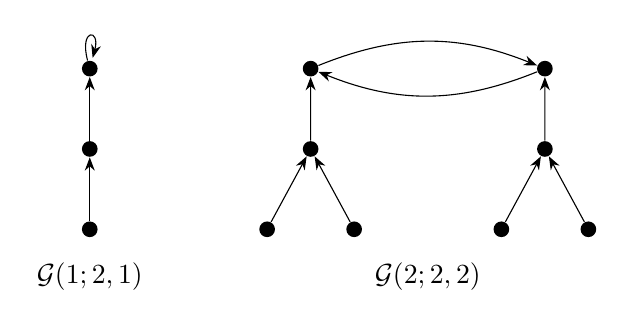
\begin{tikzpicture}[>=Stealth,vertex/.style={circle,fill=black,inner sep=2pt},
 every edge/.style={draw,->},scale=.85]
 \node[vertex] (a) at (0,0) {};
 \node[vertex] (b) at (0,-1.2) {};
 \node[vertex] (c) at (0,-2.4) {};
 \path (a) edge[loop above] (a) (b) edge (a) (c) edge (b);
 \node at (0,-3.1) {$\G(1;2,1)$};
 \node[vertex] (r) at (3.3,0) {};
 \node[vertex] (s) at (6.8,0) {};
 \node[vertex] (r1) at (3.3,-1.2) {};
 \node[vertex] (s1) at (6.8,-1.2) {};
 \node[vertex] (r2) at (2.65,-2.4) {};
 \node[vertex] (r3) at (3.95,-2.4) {};
 \node[vertex] (s2) at (6.15,-2.4) {};
 \node[vertex] (s3) at (7.45,-2.4) {};
 \path (r) edge[bend left=22] (s) (s) edge[bend left=22] (r)
 (r1) edge (r) (s1) edge (s)
 (r2) edge (r1) (r3) edge (r1) (s2) edge (s1) (s3) edge (s1);
 \node at (5.05,-3.1) {$\G(2;2,2)$};
\end{tikzpicture}
\caption{The two graph types at $n=6$. The left type occurs twice and the
right type once. Arrows indicate the induced symmetric-difference map.}
\label{fig:six}
\end{figure}

\subsection{Odd part seven}

The factorization
\[
 Q_7=(x^3+x+1)(x^3+x^2+1)
\]
gives two single-factor states $(7,1,3)$ and $(7,1,5)$, each with
polynomial $z^3-1$. For their combined support, the relations require
$3t\equiv5t\pmod7$, so the state is $(7,7,0)$, with polynomial
$(z^3-1)^2$.

At $h=1$, there are three components $\G(1;q,1)$, of masses
$2^q$, $7\cdot2^q$, and $7\cdot2^q$, and one component
$\G(7;q,1)$ of mass $49\cdot2^q$. For each dyadic $2\le h\le q$,
there are
\begin{equation}\label{eq:seven-first}
 \frac{2(2^{3h}-2^{3h/2})}{7h^2}
 \quad\text{components }\G(h;q,h),
 \qquad\text{each of mass }7h^2 2^q,
\end{equation}
and
\begin{equation}\label{eq:seven-second}
 \frac{(2^{3h}-1)^2-(2^{3h/2}-1)^2}{49h^2}
 \quad\text{components }\G(7h;q,h),
 \qquad\text{each of mass }49h^2 2^q.
\end{equation}
The number of graph types is $2a+2$.

\section{A uniform formula by fixed-point counting}\label{sec:mobius}

The preceding description uses irreducible factors and relation lattices.
A second description expresses the same partition through polynomial gcd
degrees, rotation averaging, and two M\"obius inversions. Write $\mu$ for
the integer M\"obius function and $\varphi$ for Euler's totient function.

\subsection{A bound on all cycle lengths}

For $n=qm$, define
\begin{equation}\label{eq:period-bound}
 B(n)=
 \begin{cases}
 1,&m=1,\\
 q(2^{\ord_m(2)}-1),&m>1,
 \end{cases}
\end{equation}
where $\ord_m(2)$ is the multiplicative order of $2$ modulo $m$.

\begin{lemma}\label{lem:period-bound}
Every cycle length in $\Q_n$ divides $B(n)$. For $m>1$, the larger
integer $q(2^{\varphi(m)}-1)$ may replace $B(n)$. If
$n=2^a(2^r-1)$, every cycle length divides $n$.
\end{lemma}

\begin{proof}
For $m>1$, put $r=\ord_m(2)$. On the squarefree algebra
$\F[x]/Q_m$, one has $x^{2^r}=x$, since $m\mid2^r-1$.
Hence $(1+x)^{2^r}=1+x$. As $1+x$ is invertible there,
$Q_m$ divides $(1+x)^{2^r-1}+1$. Raising this polynomial divisibility
to the $q$-th power shows
\[
 Q_m^q\mid (1+x)^{q(2^r-1)}+1.
\]
Thus $D^{B(n)}=I$ on $W_n$. A period after identifying rotations divides
an ordinary period, so the assertion follows. Euler's theorem permits
$r=\varphi(m)$ as well. When $m=2^r-1$, the same argument gives the
bound $qm=n$. If $m=1$, the periodic space is zero and the cycle length
is $1$.
\end{proof}

\subsection{The counting formula}

For every positive integer $e$, put
\begin{equation}\label{eq:Pe}
 q_e=2^{v_2(e)},\qquad m_e=e/q_e,\qquad
 P_e(X)=\left(\frac{X^{m_e}+1}{X+1}\right)^{q_e}.
\end{equation}
All polynomial gcds below are monic gcds in $\F[X]$. We use
$\gcd(P,0)=P$ and $\deg\gcd(1,f)=0$. For $k\ge1$, define
\begin{equation}\label{eq:Fe}
 F_e(k)=\frac1e\sum_{s=0}^{e-1}
 2^{\deg\gcd\left(P_e(X),(1+X)^k+X^s\right)}.
\end{equation}
For positive $d,t$, set
\begin{equation}\label{eq:Cdt}
 C(d,t)=\frac1t\sum_{e\mid d}\sum_{k\mid t}
 \mu(d/e)\mu(t/k)F_e(k).
\end{equation}

\begin{theorem}[Uniform component counts]\label{thm:mobius}
Fix $n=qm$. For $d\mid n$ and $t\mid B(n)$, $C(d,t)$ is the number
of components whose periodic coordinates have exact rotation period $d$
and whose quotient cycle has length $t$. Each such component has graph
\begin{equation}\label{eq:mobius-graph}
 \G\bigl(t;q,\gcd(d,q)\bigr)
\end{equation}
and mass $2^qdt$. All components occur in this way, and
\begin{equation}\label{eq:mobius-total}
 \sum_{d\mid n}\sum_{t\mid B(n)}2^qdt\,C(d,t)=2^n.
\end{equation}
In particular, the sums in \eqref{eq:Cdt} are nonnegative integers.
\end{theorem}

\begin{proof}
First, $F_e(k)$ counts the necklaces in the periodic part at size $e$
that are fixed by $D^k$. To see this, the kernel of multiplication by
$f$ on $\F[X]/P_e$ has dimension $\deg\gcd(P_e,f)$. For example,
writing $P_e=gP'$ and $f=gf'$ with $\gcd(P',f')=1$, the equation
$P_e\mid fu$ is equivalent to $P'\mid u$, leaving $\deg g$ free
binary coefficients. Thus each summand in \eqref{eq:Fe} counts the
periodic vectors satisfying $D^k w=R^s w$.

For a rotation orbit of size $d\mid e$ fixed by $D^k$, each of its
$d$ vectors admits exactly $e/d$ shifts $s$ modulo $e$ satisfying this
equation. The orbit contributes $e$ to the sum. An orbit not fixed by
$D^k$ contributes zero. Dividing by $e$ proves the assertion about
$F_e(k)$.

Second, repetition embeds vectors of length $e$ into length $d$ whenever
$e\mid d$. This injective map commutes with $R$ and $D$. Its image is
the set of vectors whose rotation period divides $e$, and a repeated
vector is periodic under $D$ if and only if its shorter vector is
periodic. Therefore
\[
 E_d(k)=\sum_{e\mid d}\mu(d/e)F_e(k)
\]
counts periodic necklaces of exact rotation period $d$ fixed by $D^k$.

Third, $D$ permutes these necklaces, preserving their exact rotation
period because $D$ is invertible on the periodic part and commutes with
$R$. A cycle of length $t$ contributes its $t$ vertices to $E_d(k)$
exactly when $t\mid k$. A second M\"obius inversion, followed by
division by $t$, gives \eqref{eq:Cdt}. This number is independent of
the ambient $n$ as long as $d\mid n$.

A quotient cycle with parameters $(d,t)$ contains $dt$ periodic vectors.
Attaching the full nilpotent coordinate gives one component of mass
$2^qdt$, by Theorem~\ref{thm:classification}. Its shape follows from
Theorem~\ref{thm:trees}. Lemma~\ref{lem:period-bound} includes all possible
cycle lengths. Uniqueness of the exact rotation period and quotient cycle
proves disjointness, while all periodic vectors belong to one such cycle.
This proves exhaustiveness and \eqref{eq:mobius-total}.
\end{proof}

For $h\mid q$, the multiplicity and total mass of the graph type
$\G(t;q,h)$ are therefore
\begin{align}
 M_n(t,h)&=\sum_{\substack{d\mid n\\\gcd(d,q)=h}}C(d,t),
 \label{eq:type-multiplicity}\\
 \mathcal W_n(t,h)&=2^q t
 \sum_{\substack{d\mid n\\\gcd(d,q)=h}}d\,C(d,t).
 \label{eq:type-mass}
\end{align}
A zero value of $M_n(t,h)$ means that the type is absent. By
Corollary~\ref{cor:cycle-tree}, a nonzero value requires
$h=2^{v_2(t)}$. These formulas give the complete partition in terms of
$n$, integer divisors, and polynomial gcd degrees. They do not require
specifying any subset of $X_n$.

\subsection{Mersenne widths and a prime specialization}

For $n=2^a(2^r-1)$, Lemma~\ref{lem:period-bound} allows the temporal
divisors $t\mid n$ in Theorem~\ref{thm:mobius}. In particular, at an odd
Mersenne width $m=2^r-1$, every component has type $\G(t;1,1)$ with
$t\mid m$: a cycle with one leaf attached at each cycle vertex.
The multiplicity formula determines which of these possible lengths
actually occur; a divisibility bound alone is not an occurrence assertion.

\begin{proposition}[Mersenne primes]\label{prop:mersenne-prime}
Suppose $p=2^r-1$ is prime. For $0\le s<p$, put
\[
 a_s=\deg\gcd\left(Q_p(X),X^s+X+1\right),\qquad
 A_p=\frac1p\sum_{s=0}^{p-1}(2^{a_s}-1).
\]
There are $1+A_p$ components of type $\G(1;1,1)$ and
\begin{equation}\label{eq:mersenne-prime}
 \frac{2^{p-1}-1-pA_p}{p^2}
\end{equation}
components of type $\G(p;1,1)$. Among the former, one has mass $2$
and the remaining $A_p$ have mass $2p$. Each latter component has mass
$2p^2$. For $p=3$, only the first type occurs; for $p\ge7$, both occur.
\end{proposition}

\begin{proof}
The only possible quotient cycle lengths are $1$ and $p$. Every nonzero
periodic vector has rotation period $p$, since the rotation-fixed vectors
at odd width are zero and the constant-one vector, and the latter maps
to zero under $D$. By \eqref{eq:Fe}, $A_p$ is the number of nonzero
periodic necklaces fixed by $D$. These give $A_p$ components of mass
$2p$, besides the zero-core component of mass $2$. The remaining
$2^{p-1}-1-pA_p$ periodic vectors lie in joint orbits of size $p^2$,
giving \eqref{eq:mersenne-prime}.

The case $p=3$ follows from Table~\ref{tab:three-five}. For $p\ge7$,
consider the full annihilator $Q_p$. Its quotient cycle cannot have
length $1$: that would require $1+X=X^s\pmod{Q_p}$ for some
$0\le s<p$. The nonzero polynomial $X^s+X+1$ has degree at most
$p-1$. If its degree is smaller, $Q_p$ cannot divide it. If its degree
is $p-1$, it has three nonzero terms, whereas
$Q_p=1+X+\cdots+X^{p-1}$ has $p$ terms. Thus its quotient cycle has
length $p$, proving existence of the second type. The zero-core component
always gives the first.
\end{proof}

\section{Consequences and further questions}\label{sec:questions}

The partition separates three kinds of information. The isomorphism type
is determined by $(n,T)$ through \eqref{eq:cycle-tree}. Its multiplicity
is an orbit count, given by \eqref{eq:tower-multiplicity} or
\eqref{eq:type-multiplicity}. Its mass retains spatial-period information
that the unweighted graph may lose. Accordingly, a classification of graph
types alone does not determine the cardinalities of all parts of the power
set. The coset description and mass formulas retain the additional data.

For fixed odd $m$, Theorem~\ref{thm:tower} gives a finite algebraic
description of an infinite family. Increasing the exponent of $2$ changes
the nilpotent depth and the dyadic lattice scale, while the squarefree
relation lattices remain fixed. This explains why the number of graph
types is linear in $a$, even though the power set has $2^{m2^a}$ elements.

Several questions arise naturally from this formulation. They are stated
as directions for further study, without a claim that each is unresolved
in the existing literature.

\begin{enumerate}
\item \textbf{Arithmetic of the odd part.}
Can the set $\mathcal S_m$ of quotient cycle lengths be characterized
directly from arithmetic properties of $m$, beyond its definition by
supports of irreducible factors? Such a characterization would describe
which graph types occur throughout the family $m2^a$.

\item \textbf{Occurrence at Mersenne widths.}
For $m=2^r-1$, which divisors $t\mid m$ satisfy
$\sum_{d\mid m}C(d,t)>0$? The formula in
Theorem~\ref{thm:mobius} determines the answer, but a structural
criterion for positivity would expose additional arithmetic information.

\item \textbf{Weighted graph classification.}
For a prescribed graph type at fixed $n$, what are the possible component
masses, and with what multiplicities do they occur? Here the relevant
distinction is among the values of $d$ contributing to
\eqref{eq:type-mass}, even when the cycle length and tree are fixed.

\item \textbf{Other local maps.}
For maps given by other polynomials in $R$, which rotation quotients have
level-regular attached trees, and when do their joint relation lattices
admit an equally simple lifting law? The derivative argument in
\eqref{eq:derivative} identifies a specific feature of the pair $x,1+x$
that a generalization must address.
\end{enumerate}

The central classification is independent of these further questions.
For every $n$, the annihilator and coset construction gives a disjoint
partition of the power set, the tree theorem gives each graph explicitly
up to isomorphism, and the counting identities account for all $2^n$
subsets. The finite polynomial data for an odd part describe all of its
doublings simultaneously.

\begin{thebibliography}{9}

\bibitem{MartinOdlyzkoWolfram}
O.~Martin, A.~M.~Odlyzko, and S.~Wolfram,
\emph{Algebraic properties of cellular automata},
Communications in Mathematical Physics \textbf{93} (1984), no.~2,
219--258.
\href{https://doi.org/10.1007/BF01223745}{doi:10.1007/BF01223745}.

\bibitem{MisiurewiczStevensThomas}
M.~Misiurewicz, J.~G.~Stevens, and D.~M.~Thomas,
\emph{Iterations of linear maps over finite fields},
Linear Algebra and its Applications \textbf{413} (2006), no.~1,
218--234.
\href{https://doi.org/10.1016/j.laa.2005.09.002}{doi:10.1016/j.laa.2005.09.002}.

\bibitem{BreuerLotterMerwe}
F.~Breuer, E.~L\"otter, and B.~van der Merwe,
\emph{Ducci-sequences and cyclotomic polynomials},
Finite Fields and Their Applications \textbf{13} (2007), no.~2,
293--304.
\href{https://doi.org/10.1016/j.ffa.2005.11.003}{doi:10.1016/j.ffa.2005.11.003}.

\end{thebibliography}
\end{document}
